\documentclass[11pt]{article}
    
\usepackage{amsmath}
\usepackage{amsfonts}
\usepackage{cite}
\usepackage[letterpaper, total={6.5in, 9in}]{geometry}
\usepackage{mathpazo}
\usepackage{sourcecodepro}
\usepackage{graphicx}
\usepackage{hyperref}
\usepackage[title]{appendix}

\newcommand{\setcomp}[2]{\left\{ #1 \ \Big|\ #2 \right\}}
\newcommand{\rngto}[1]{1{:}#1}
\newcommand{\abs}[1]{\left| #1 \right|}
\newcommand{\absdet}[1]{\abs{#1}}
\newcommand{\dv}[1]{\mathrm{d}{#1}}
\newcommand{\Exp}{\mathrm{Exp}}
\newcommand{\vect}{\mathrm{vec}}
\newcommand{\vectu}{\mathrm{vecu}}

\begin{document}


\title{Efficient Unconstraining
  Parameter Transforms for Hamiltonian Monte Carlo}
\author{Meenal Jhajharia \\ \small Flatiron Institute 
\and Seth Axen \\ \small University of T\"ubingen 
\and Adam Haber \\ \small Weizmann Institute 
\and Sean Pinkney \\ \small Omnicom Media Group
\and Bob Carpenter \\ \small Flatiron Institute}
\date{DRAFT: \today}
\maketitle

\begin{abstract}
  \noindent
  This paper evaluates the statistical and computational
  efficiency of unconstraining parameter transforms for Hamiltonian
  Monte Carlo sampling.
\end{abstract}

\section{Introduction}

In statistical computing, we often need to compute high-dimensional
integrals over densities $\pi(x)$ (e.g., Bayesian estimation or
prediction, $p$-value calculations, etc.).  The only black-box
techniques that work for general high-dimensional integrals are
Markov chain Monte Carlo (MCMC) methods.  The most effective MCMC
method in high dimensions is Hamiltonian Monte Carlo (HMC).  HMC works
by simulating the Hamiltonian dynamics of a fictitious particle
representing the value being sampled coupled with a momentum term.

Although it is possible to write HMC samplers that work for simply
constrained values such as upper- and/or lower-bounds
\cite{neal2011mcmc} or unit vectors \cite{byrne2013geodesic}, it is
much more challenging to do the same for complex constraints such as
simplexes or positive definite matrices or for densities involving
multiple constrained values.  Instead, it is far more common to map
the constrained values to unconstrained values before sampling
\cite{JSSv076i01}.  For example, the Probabilistic  Programming language Stan, defines distributions with an unconstrained support, in favour of making sampling an easier process. The variables with constraints (or with constrained support in this case) are transformed to an unconstrained space. Inverse transforms of these variables are used for log density adjustments. These are usually in the form of a Jacobian matrix comprised of the gradient $\frac{\partial x}{\partial y}$, where $x$ and $y$ are the constrained and unconstrained parameters respectively.

These gradients are computationally expensive, certain transforms are entirely inefficient, and some work well on certain distributions or parametrizations and vice versa. This presents the issue of selecting which transform to use
among an infinite set of options, which is the topic of this paper. We begin by defining the general theory of transforms, followed by transforms from a unit simplex $\Delta^N$ to the $R^M$. Finally, we discuss notions of "better" transforms defined on the simplex, using statistical measures like Effective Sample Size, Leapfrog steps taken by the sampler etc.




\section{Unconstraining Transforms}

To draw samples from a parameter defined on a constrained space $\mathcal{X}$ that can be uniquely parameterized by $n$ real degrees of freedom, we instead perform sampling in an unconstrained space $\mathcal{Y} \in \mathbb{R}^m$ for $m \ge n$. Let $p_Y(y)$ be an improper density function defined over $\mathcal{Y} \rightarrow(0, \infty)$ with support over all elements of $\mathcal{Y}$ and a surjective, smooth and continuous map $g: \mathcal{Y} \rightarrow \mathcal{X}$. Then, for any proper density $\pi_{X}$ over $\mathcal{X}$, the constraining transform can be defined as $\left(p_{Y}, g\right)$: $\mathcal{Y} \rightarrow \mathcal{X}$. In this case, the density $p_{Y}(y)=\pi_{Y}(y) \cdot \pi_{X}(g(y))$ is proper, and $Y \sim \pi_Y \implies g(Y) \sim \pi_X$. The required change of variables for this unconstraining transform is:
\[
  p_Y(y) = p_X(f^{-1}(y)) \absdet{J_{f^{-1}}(y)},
\]
where the Jacobian of the inverse transform is defined by
\[
  J_{f^{-1}}(y) = \frac{\partial}{\partial y} \, f^{-1}(y)
\]

%notion of uniformity missing
In this paper we consider transforms where $m = n$, for which the constraining transform is defined as $(\pi_Y, f)$: $\mathcal{Y} \rightarrow \mathcal{X}$, given that $\pi_{Y}(y)=\absdet{J_{f^{-1}}(y)}$.



\section{Unit simplex}

A unit $N$-simplex is an $N + 1$-dimensional vector of non-negative
values that sums to one.  Simplexes are useful for representations of multinomial probabilities
(e.g., probabilities of categories in a classification problem). The set of unit $N$-simplexes is conventionally denoted
\[
  \Delta^N = \setcomp{x \in \mathbb{R}_{\ge 0}^{N + 1}}{ \sum_{i=1}^{N} x_i = 1}
\]
Geometrically, an $N$-simplex is the convex closure of $N+1$ points
that are 1 in one coordinate and 0 elsewhere.  For example, the
3-simplex is the complex closure of
$\begin{bmatrix}1 & 0 & 0 \end{bmatrix},
\begin{bmatrix} 0 & 1 & 0 \end{bmatrix}$,
and $\begin{bmatrix} 0 & 0 & 1 \end{bmatrix}$. As such, there are only $N$ degrees of
freedom, because if $x$ is an $N$-simplex, then
\[
  x_N = 1 - (x_1 + x_2 + \cdots + x_{N-1}).
\]
%n not n-1
We will use $\Delta^N_-$ to denote $N$ elements of a simplex, this is sufficient to uniquely determine $\Delta^N$.
\subsection{Stick-Breaking Transform}

The Stick-Breaking transform carries forward the intuition in the stick-breaking construction for Dirichlet \cite{sethuraman1994constructive}. It is a process of recursively breaking a piece $x_i$ from a stick of unit length, where the leftover stick in the $i^{th}$ iteration is $ 1 - \sum_{1}^{i}x$. Let $y = f(x)$, then we define the stick-breaking mapping $ f \colon \Delta^{N-1} \to  R^{N-1}$, for $1 \leq i \leq N$ as:	
\[
y_i
= \mathrm{logit}(z_i) - \mbox{log}\left(\frac{1}{N-i}
   \right) 
   \]
  
for break proportion 
\[ 
 z_i = \frac{x_i}{1 - \sum_{i' = 1}^{i-1} x_{i'}}.
\]\\

The inverse transform $ f^{-1} \colon R^{N-1} \to \Delta^{N-1}$ is defined as:

\[
x_i = \left( 1 - \sum_{i'=1}^{i-1} x_{i'} \right)\\
\]

for break proportion \[z_i = \mathrm{logit}^{-1} \left( y_i  + \log \left( \frac{1}{N - i}
                                            \right)\right)
                                            \]\\
                                            
The determinant of the Jacobian
\[
   \abs{\mathbf{J}} = \prod_{i=1}^{N-1}z_i\,(1 - z_i)\left(1 - \sum_{i'=1}^{i-1} x_{i'}\right)
\]
\subsection{Additive log ratio transform}
The unconstraining transform for the identified softmax is known as
the additive log ratio (ALR) transform
\cite{aitchison1982statistical}, which is a bijection
$\textrm{alr}:\Delta^{N-1} \rightarrow \mathbb{R}^{N-1}$ defined for
$x \in \Delta^{N-1}$ by
\[
  \textrm{alr}(x)
  = \begin{bmatrix}\displaystyle
    \log \frac{x_1}{x_N} \cdots \log \frac{x_{N-1}}{x_N}
  \end{bmatrix}
\]
The inverse additive log ratio transform maps values in
$\mathbb{R}^{N-1}$ to $\Delta^{N-1}$ defined for $y \in
\mathbb{R}^{N-1}$ by
\[
  \textrm{alr}^{-1}(y)
  = \textrm{softmax}(\begin{bmatrix} y &  0 \end{bmatrix}),
\]
where for $u \in \mathbb{R}^N$,

\[
  \textrm{softmax}(u) = \frac{exp(u)}{\sum exp(u)}
\]

\[
\textrm{Here, } \abs{J} = \prod \exp(y)
  \, \left( \frac{1}{1 + \sum(\exp(y))} \right)^N
\]
\subsection{Augmented-Softmax Transform}
% Needs to be written like other transforms -> transform, inverse, |J|
We define the transformation
$\phi: \mathbb{R}^n \to \Delta^{N} \times \mathbb{R}_{>0}: y \mapsto
(x_-, r)$, where  $\Delta_{-}^N$ and $x_{-}$  denote $N$ elements of the simplex and $x$, respectively. Here $r = \sum_{i=1}^n \textrm{exp}(y_i)$,
$x_i = \frac{1}{r} \textrm{exp}(y_i)$ for $i \in [1, N-1]$ and $\delta_{ij}$ is the Kronecker delta function. If $\mathrm{diag}(x)_{i, j} = \delta_{ij} x_i$ and $\boldsymbol{1}_n$ is the $N$-vector of ones.\[
  J = (I_{N-1} - x_- \boldsymbol{1}_{N-1}^\top) \operatorname{diag}(x_-),
\] 

Using Sylvester's determinant theorem,
$|I_{N-1} - x_- \boldsymbol{1}_{N-1}^\top| = 1 -
\boldsymbol{1}_{N-1}^\top x_- = 1 - \sum_{i=1}^{N-1} x_i = x_N$, so
$$ |J| = x_n \prod_{i=1}^{N-1} x_i = \prod_{i=1}^{N} x_i = \exp\left(\sum_{i=1}^{N-1} y_i\right) \left(1 + \sum_{i=1}^{N-1} e^{y_i}\right)^{-N}$$

\section{Results}
\begin{figure}[h!]
    \centering
    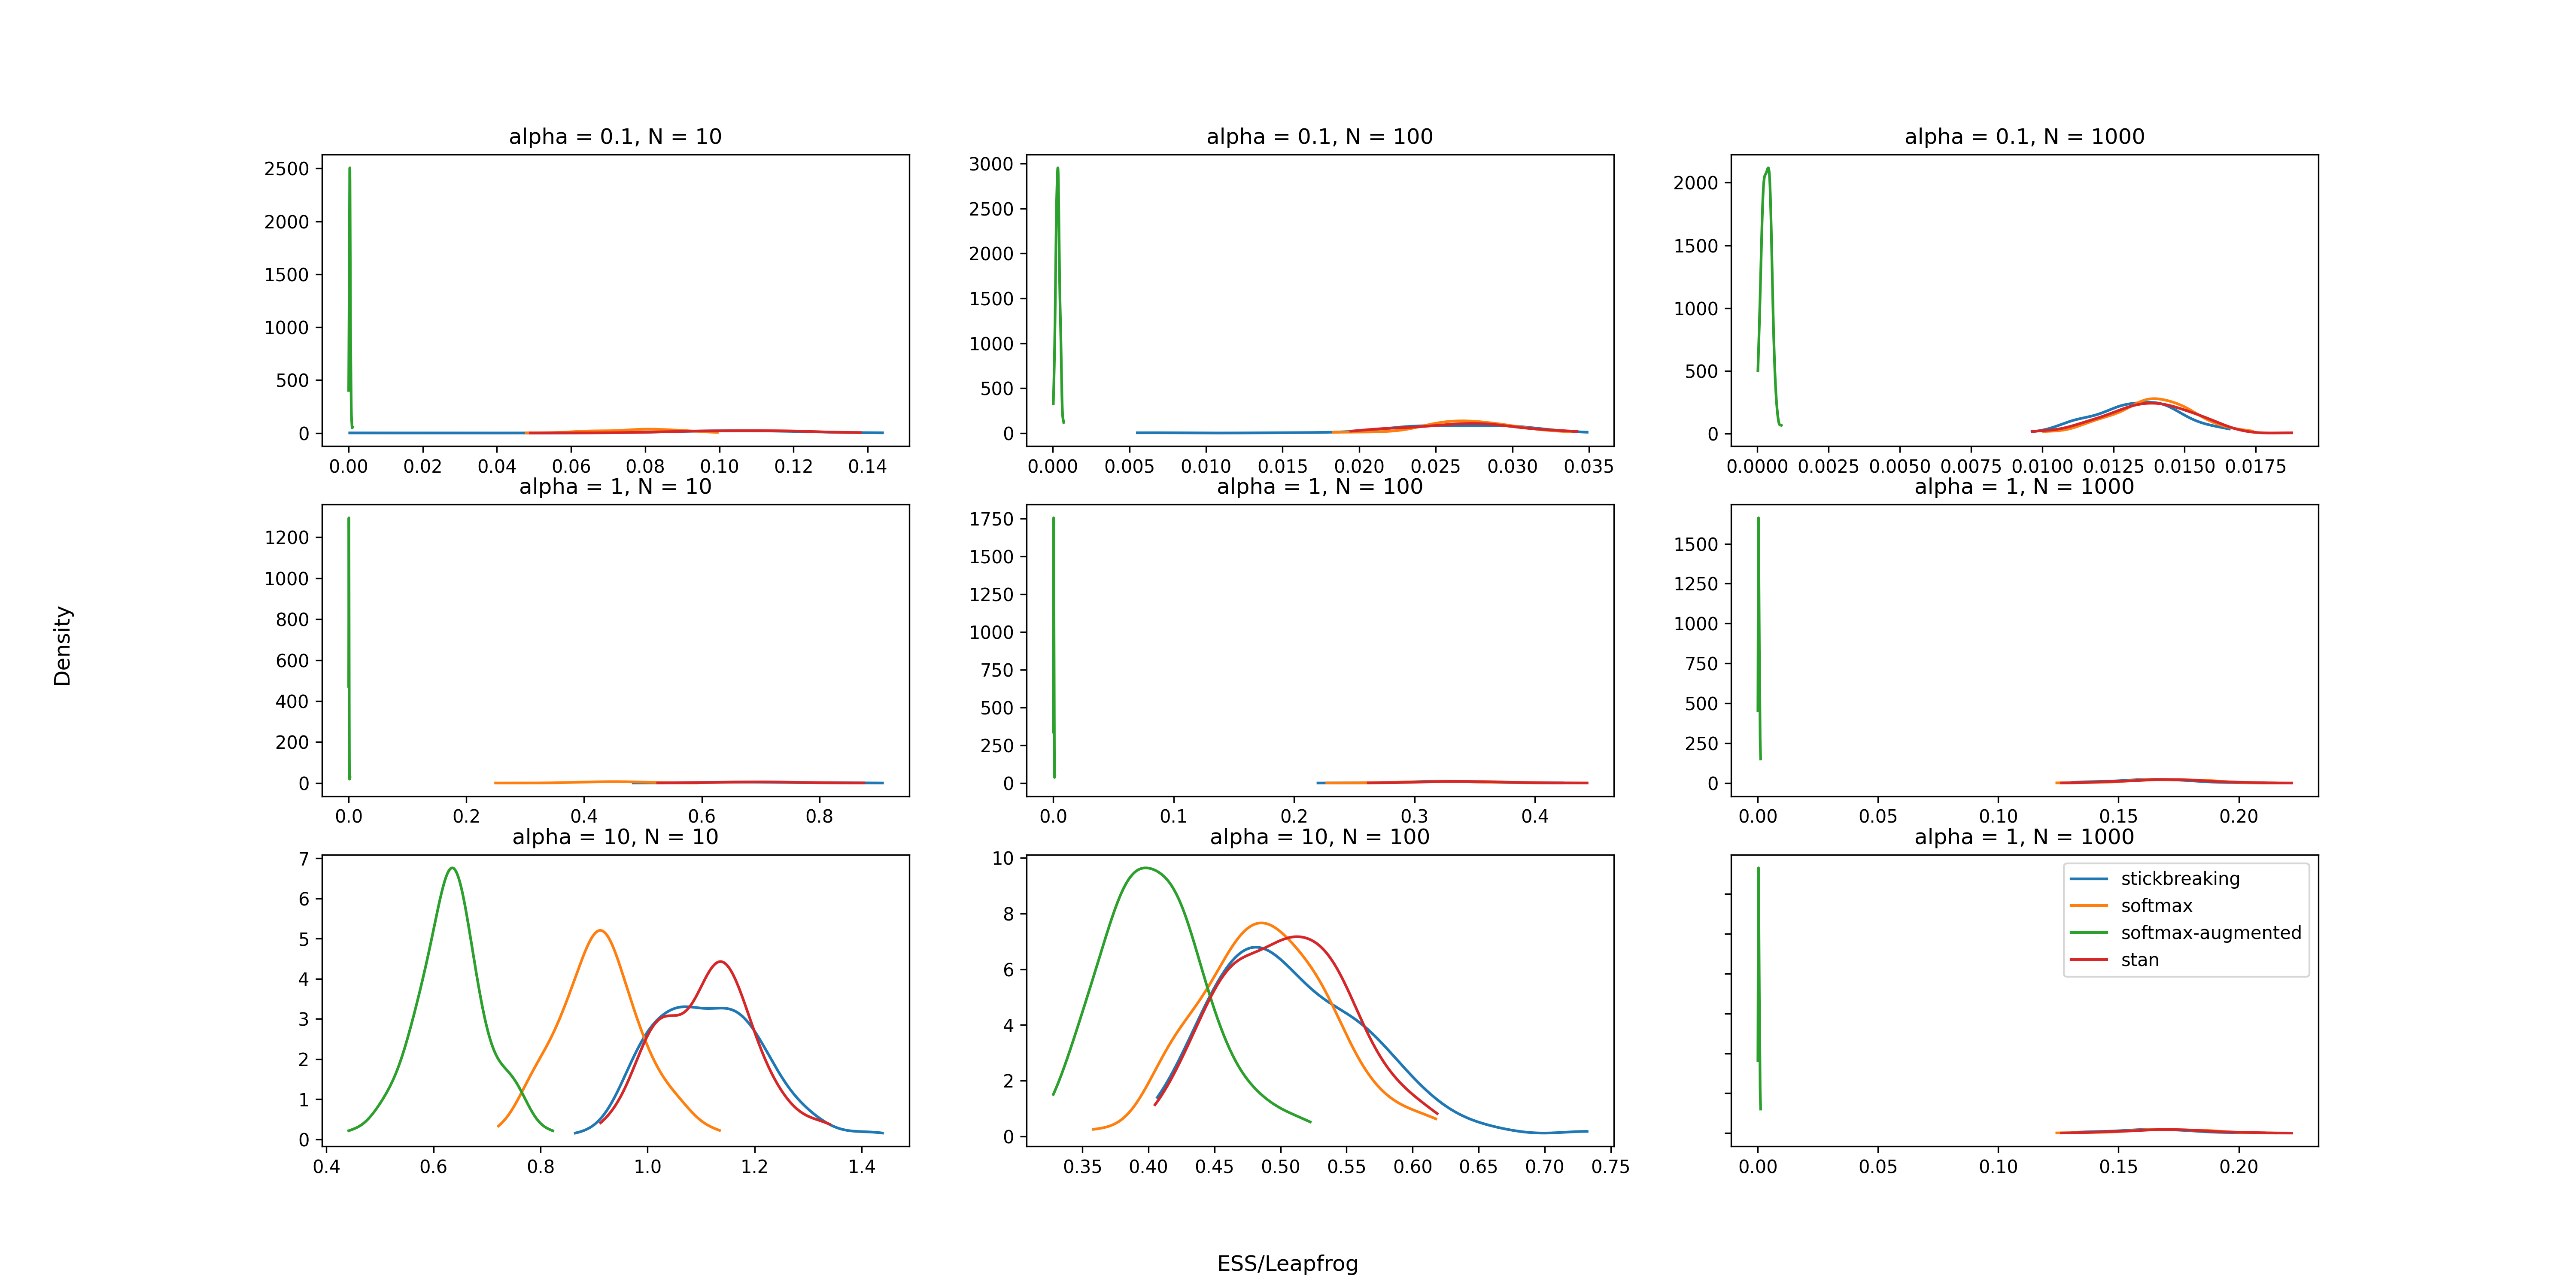
\includegraphics[width=1.2\textwidth]{figures/simplex/ess_density.png}
    \caption{Probability Density plot of Effective Sample Size/Total LeapFrog Steps. Effective sample size is evaluated at 100 runs, each point is the value of ESS/Total Leapfrog steps taken by the sampler in one run.}
    \label{fig:ess_density}
\end{figure}
\newpage
\begin{figure}[h!]
    \centering
    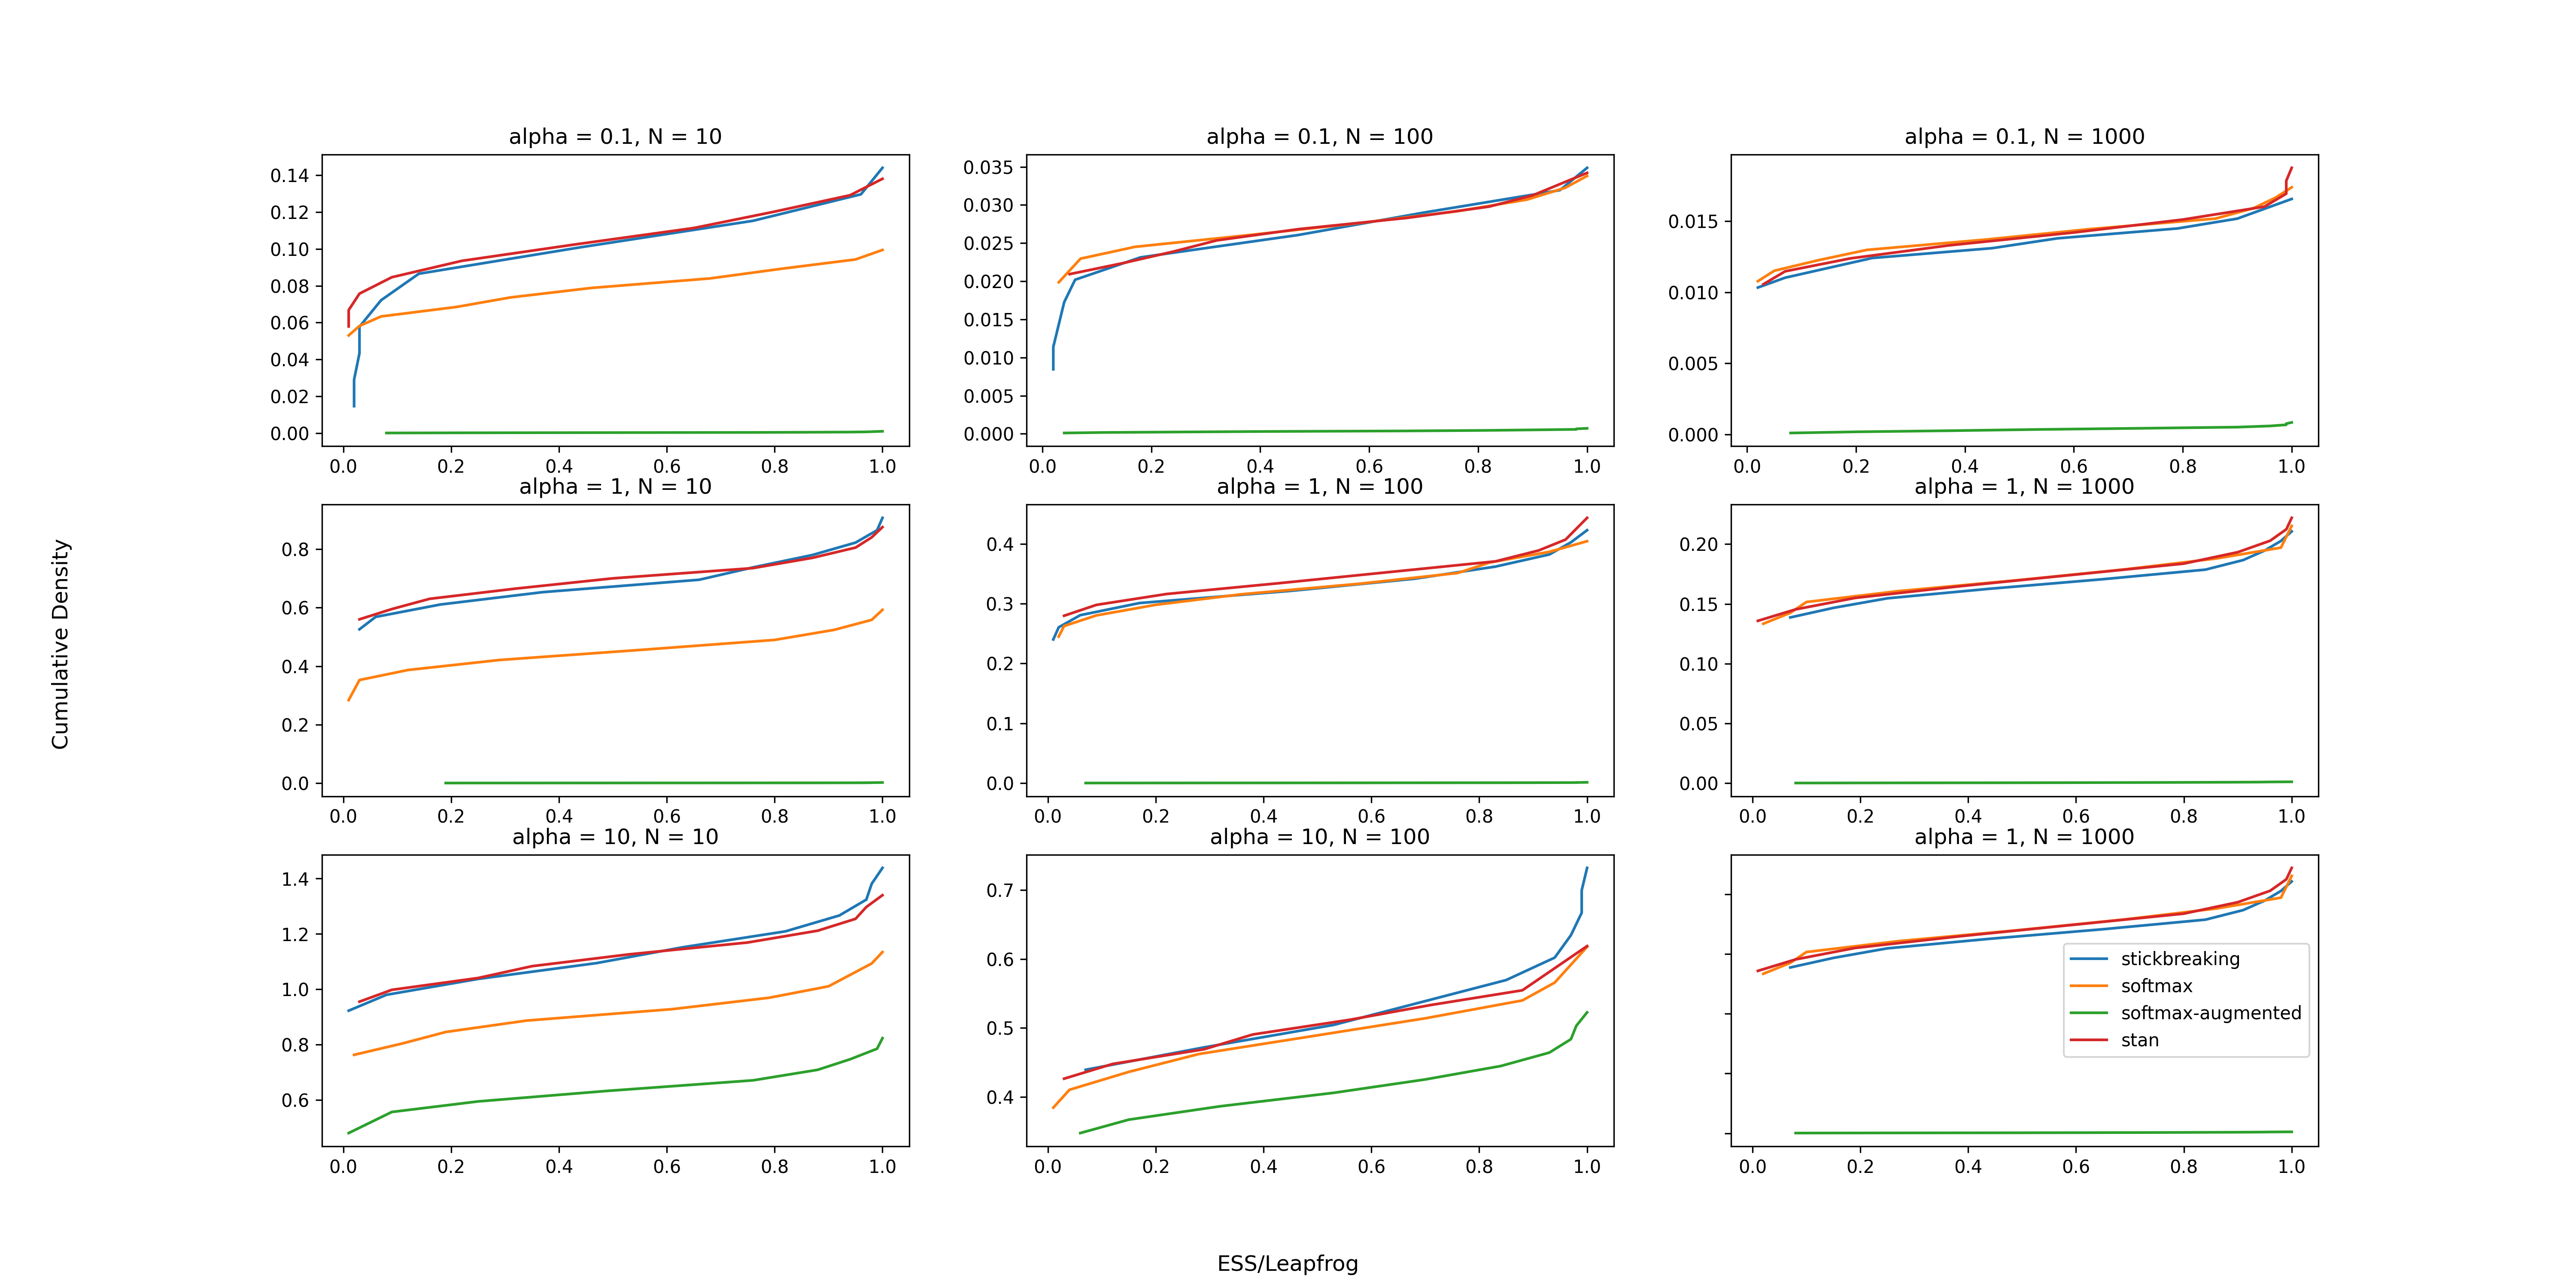
\includegraphics[width=1.2\textwidth]{figures/simplex/ess_cdf.png}
    \caption{Cumulative Density plot of Effective Sample Size/Total LeapFrog Steps. Effective sample size is evaluated at 100 runs, each point is the value of ESS/Total Leapfrog steps taken by the sampler in one run.}
    \label{fig:ess_cdf}
\end{figure}

\begin{figure}[h!]
    \centering
    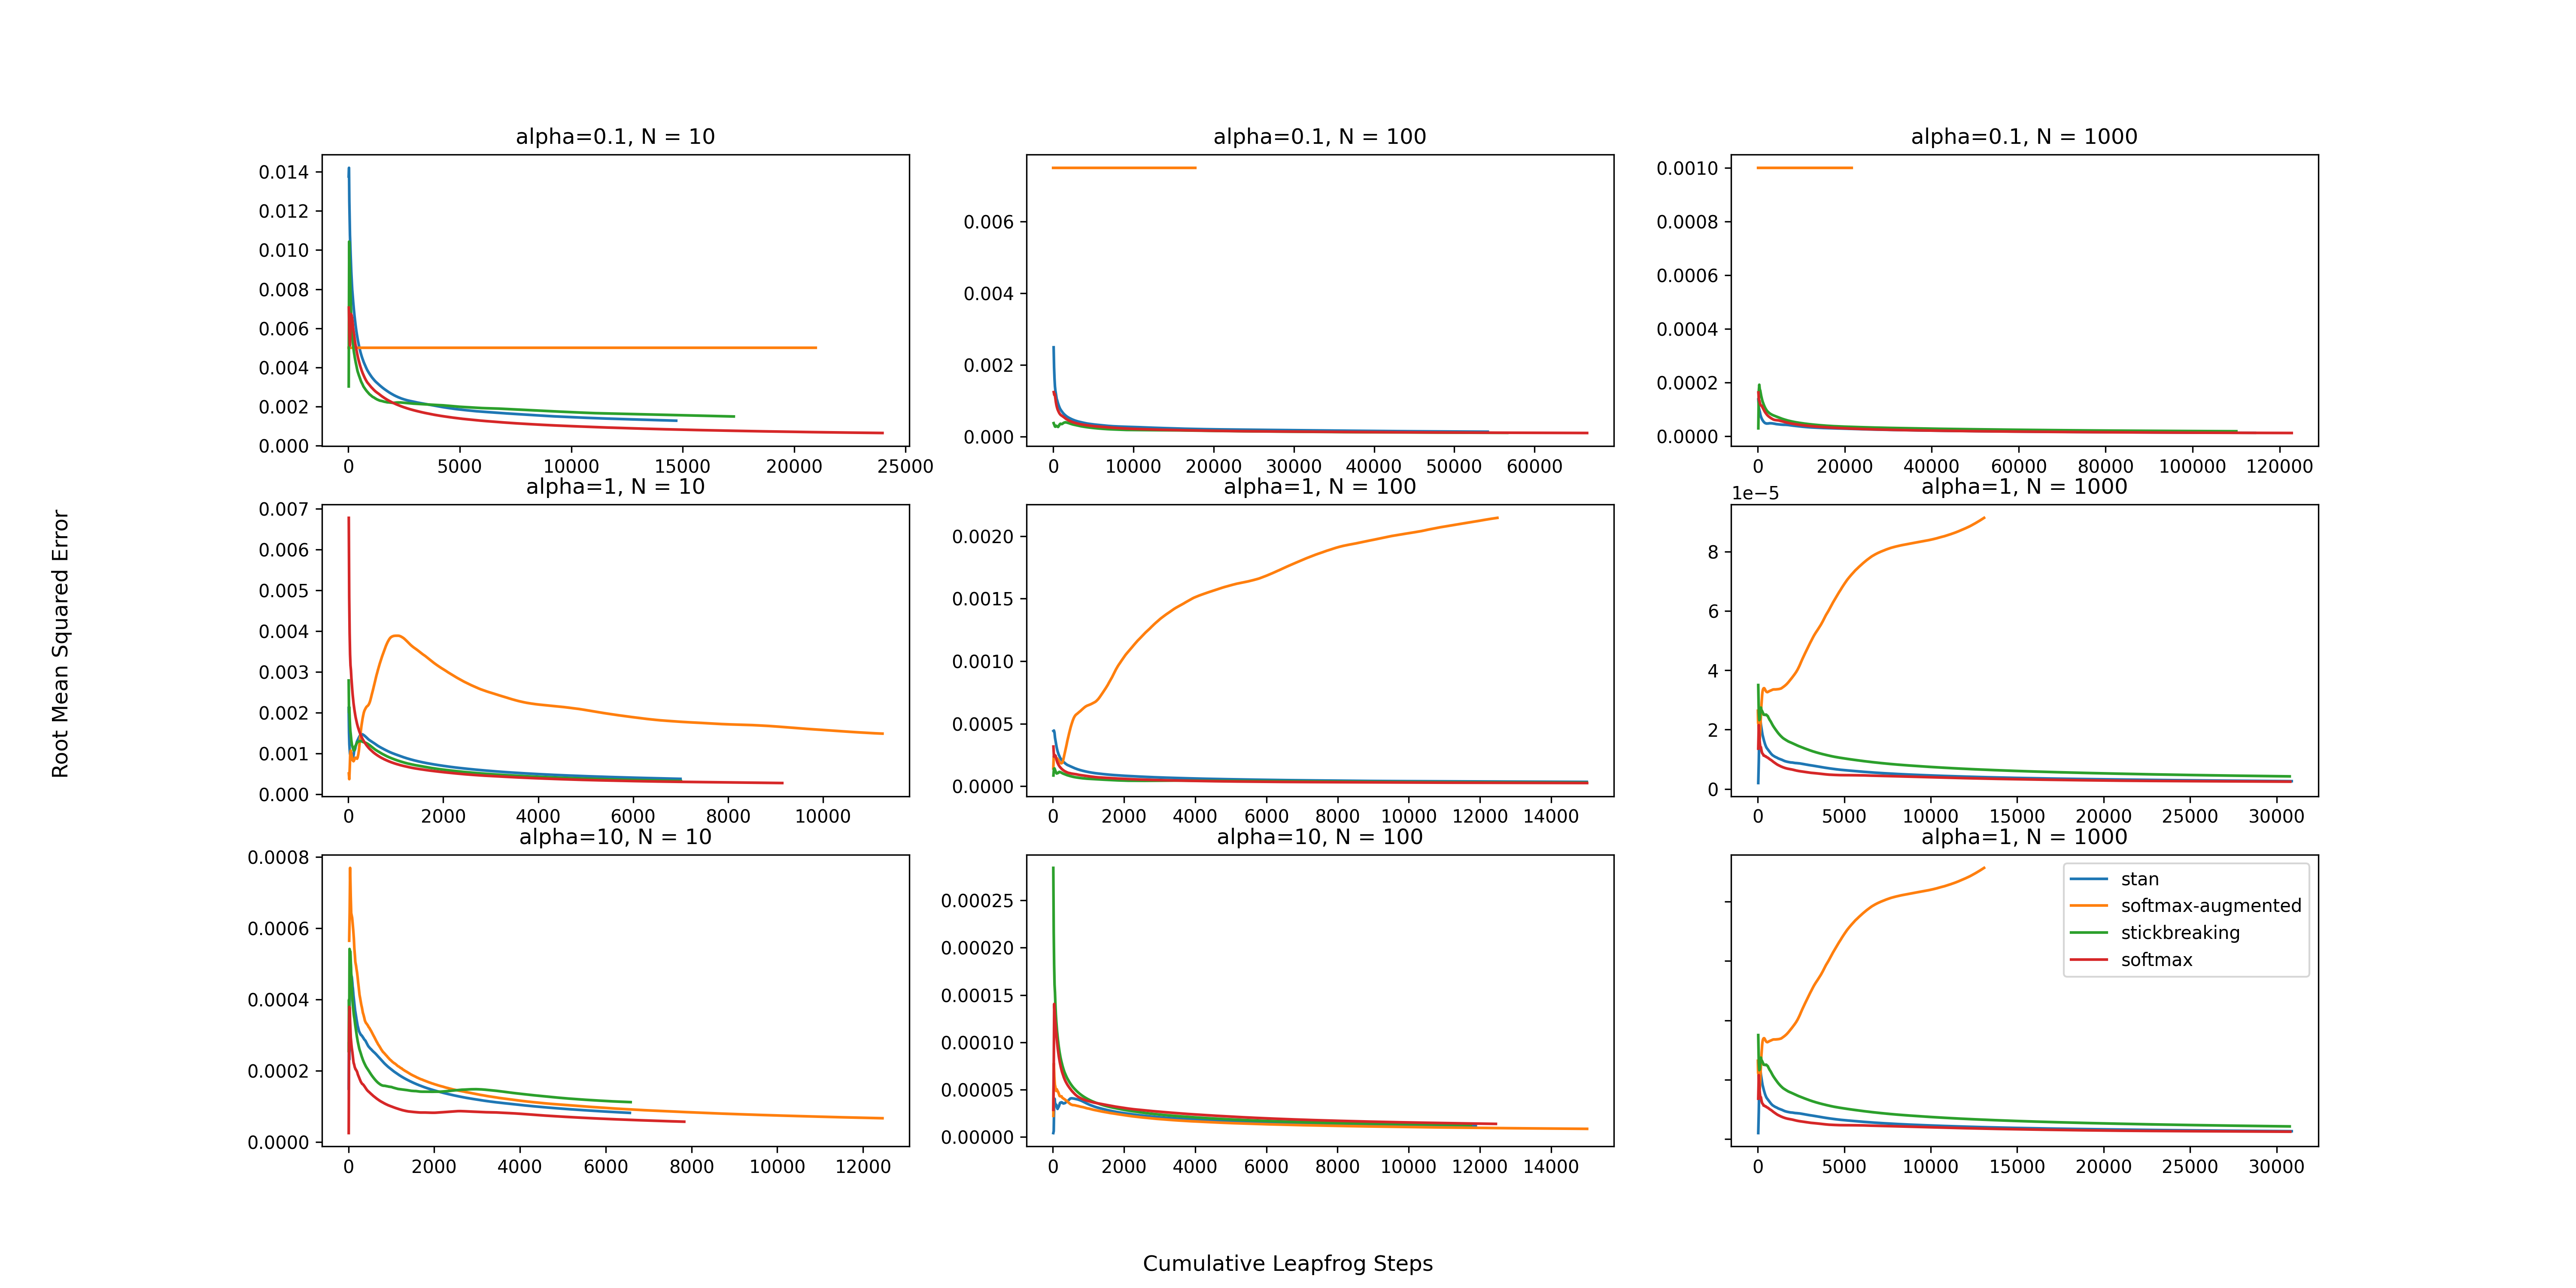
\includegraphics[width=1.2\textwidth]{figures/simplex/rmse.png}
    \caption{Root Mean Squared Error vs Cumulative Leapfrog Steps. At every iteration in a run, cumulative mean of samples is used to calculate RMSE, which is plotted against the cumulative leapfrog steps till that iteration}
    \label{fig:rmse}
\end{figure}
\clearpage
\subsubsection*{Acknowledgements}

We would like to thank \url{matrixcalculus.org} for providing an
easy-to-use symbolic matrix derivative calculator.



\bibliography{all}{}
\bibliographystyle{plain}

\begin{appendices}

\section{Jacobian Determinants}
\subsection{Stickbreaking Transform}
The Jacobian matrix for $f^{-1}$ is a lower-triangular diagonal matrix, so for the change of variables we evaluate $\mathbf{J}_{i, i}$ where $i \in 1:N-1$.
\begin{align*}
\mathbf{J}_{i, i} &= \frac{\partial x_i}{\partial y_i}
=
\frac{\partial x_i}{\partial z_i} \,
\frac{\partial z_i}{\partial y_i}\\
\mathbf{J}_{i, i} &= \left(
  1 - \sum_{k' = 1}^{k-1} x_{k'}
   \right) z_k (1 - z_k),\\
   \abs{\textbf{J}} &= \prod_{i=1}^{N-1} \textbf{J}_{i,i}
\end{align*}

The change of variables adjustment $p_Y(y) = p_X(f^{-1}(y))\,
\prod_{i=1}^{N-1}z_i\,(1 - z_i)\left(1 - \sum_{i'=1}^{i-1} x_{i'}\right).$

\subsection{Additive Log ratio transform}
To calculate the determinant of the Jacobian of the inverse transform,
we start by noting that $s = \textrm{exp} \circ \textrm{norm}$, where
$\textrm{exp}$ is the elementwise exponential function and
\textrm{norm} is defined by
\[
  \textrm{norm}(z) = \frac{z}{\textrm{sum}(z) + 1}.
\]
As such, the resulting Jacobian determinant is the product of the
Jacobian determinants of the component functions,
\[
  \absdet{J_s(y)}
  = \absdet{J_{\textrm{exp}}(y)} \absdet{J_{\textrm{norm}}(z)},
\]
where $z = \textrm{exp}(y)$.  The Jacobian for the exponential
function is diagonal, so the determinant is the product of the
diagonal of the Jacobian, which for $y \in \mathbb{R}^{N-1}$ is
\[
  \absdet{J_{\textrm{exp}}(y)} = \textrm{prod}(\exp(y)).
\]
As above, let $z = \exp(y) \in (0, \inf)^{N-1}$.  We can differentiate
$\textrm{norm}$ to derive the Jacobian,
\[
  J_{\textrm{norm}}
  = \frac{1}{1 + \textrm{sum}(z)} \mathbb{I}_{N-1}
  - \left(\frac{1}{(1 + \textrm{sum}(z))^2} \beta \right)
  \textrm{vector}_{N-1}(1)^{\top},
\]
where $\mathbb{I}_{N-1}$ is the $(N - 1) \times (N - 1)$ unit matrix and
$\textrm{vector}_{N-1}(1)$ is the $N - 1$-vector with values 1.  Using
the matrix determinant lemma,\footnote{The matrix determinant lemma
  is \[\textrm{det}(A + u v^{\top}) = (1 + v^{\top} A^{-1} u)
    \textrm{det}(A).\]}
we have
\begin{eqnarray*}
  \textrm{absdet}(J_{\textrm{norm}}(z))
  & = &
  \left(
    1
    + \textrm{vector}_{N-1}(1)^{\top}
    \left(\frac{1}{1 + \textrm{sum}(z)} \mathbb{I} \right)^{-1}
    \frac{-z}{(1 + \textrm{sum}(z))^2}
    \right)
    \ \textrm{det}\left(\frac{1}{1 + \textrm{sum}(z)} \mathbb{I}
        \right)
  \\[6pt]
  & = &
  \left(
    1 
    + \textrm{sum}\left( \frac{-(1 + \textrm{sum}(z)) z}{(1 +
        \textrm{sum}(z))^2} \right)
  \right)
        \ \left( \frac{1}{1 + \textrm{sum}(z)} \right)^{N-1}
  \\[6pt]
  & = &
        \left(1 + \textrm{sum}\left(\frac{-z}{1 + \textrm{sum}(z)} \right)\right)        
        \ \left( \frac{1}{1 + \textrm{sum}(z)} \right)^{N-1}
  \\[6pt]
  & = & \left( 1 - \textrm{sum}(\textrm{norm}(z)) \right) 
        \ \left( \frac{1}{1 + \textrm{sum}(z)} \right)^{N-1}
  \\[6pt]
  & = & \left( \frac{1}{1 + \textrm{sum}(z)} \right)^N.
\end{eqnarray*}
Thus the entire absolute determinant of the Jacobian is defined by the
product, 
\[
  \absdet{J_s(y)}
  \ = \
  \textrm{prod}(\exp(y))
  \, \left( \frac{1}{1 + \textrm{sum}(\exp(y))} \right)^N.
\]
and our final expression for densities for unconstrained $y \in
\mathbb{R}^{N-1}$ is
\[
  p_Y(y)
  = p_X(\textrm{alr}^{-1}(y))
  \, \textrm{prod}(\exp(y))
  \left( \frac{1}{1 + \textrm{sum}(\exp(y))} \right)^N
\]

\subsection{Hyperspherical simplex transforms}

\subsubsection{Hyperspherical coordinate transform}

We use the following definition of hyperspherical coordinates.
For $\phi_i \in (0, \pi/2]$ and $u \in \mathbb{S}^N_{>0}$, the positive orthant of the $N$-sphere,
\[
  u_i = \left(\prod_{k=1}^{i-1} \sin(\phi_k)\right) \begin{cases}
    1 & \text{ if } i = N + 1\\
    \cos(\phi_i) & \text{otherwise}
  \end{cases}.
\]

Let $z_i = \sin^2(\phi_i)$ and $x_i = u_i^2$, so that $x \in \Delta^N$.
Then
\[
  x_i = \left(\prod_{k=1}^{i-1} z_k\right) \left(\begin{cases}
    1 & \text{ if } i = N + 1\\
    (1 - z_i) & \text{otherwise}
  \end{cases}\right) = (1 - z_i (1 - \delta_{i,N+1})) \prod_{k=1}^{i-1} z_k.
\]

\subsubsection{Hyperspherical coordinates inverse transform}

To derive the inverse transform, note that
\[
    \begin{aligned}
        x_{N+1} &= \prod_{k=1}^{N} z_k\\
        x_N + x_{N+1} &= (1 - z_N)\left(\prod_{k=1}^{N-1} z_k\right) + z_N \left( \prod_{k=1}^{N-1} z_k \right) = \prod_{k=1}^{N-1} z_k = \frac{x_N}{1 - z_N}\\
        x_{N-1} + x_{N} + x_{N+1} &= (1-z_{N-1}) \left(\prod_{k=1}^{N-2} z_k\right) + z_{N-1} \left(\prod_{k=1}^{N-2} z_k\right) = \prod_{k=1}^{N-2} z_k = \frac{x_{N-1}}{1 - z_{N-1}}\\
        &\vdots \\
        \sum_{k=i}^{N+1} x_{k} &= \prod_{k=1}^{i - 1} z_k = \frac{x_i}{1 - z_i}.
    \end{aligned}
\]

From the final expression, we can define the inverse transform:
\[
z_i = 1 - \frac{x_i}{\sum_{k=i}^{N+1} x_k}
\]

\subsubsection{Jacobian of hyperspherical coordinates transform}

To derive the Jacobian, we note that $x_i$ depends only on $z_k$ for $k \le i$.
As a result, the Jacobian of the map from $z$ to $x_-$ is lower triangular, and its determinant depends only on its diagonal, which consists of the terms
$$J_{ii} = -\frac{\partial x_i}{\partial z_i} = \prod_{k=1}^{i-1} z_k,$$
so
$$
|J| = \prod_{i=1}^N |J_{ii}|
= \prod_{i=1}^N \prod_{k=1}^{i-1} z_k
= \prod_{k=1}^{N-1} \prod_{i=k+1}^N z_k
= \prod_{i=1}^{N-1} z_i^{N-i} = \prod_{i=1}^N z_i^{N-i}
$$

Due to the form of the Jacobian correction, if $x$ is uniformly distributed on the unit simplex, then $z_i$ and $z_j$ are uncorrelated for all $i \ne j$.

\subsubsection{Hyperspherical angular transform}

The map from $y$ to $z$ is elementwise, so its Jacobian is diagonal.
Each element is
$$\sin^{-1}(\sqrt{z_i}) = \phi_i = \frac{\pi}{2} \operatorname{logit}^{-1} (y_i).$$
Differentiating all sides with respect to $y_i$, we find
$$
\begin{aligned}
\frac{1}{\sqrt{1 - z_i^2}} \frac{1}{2 \sqrt{z_i}} \frac{\partial z_i}{\partial y_i} &= \frac{\pi}{2} \operatorname{logit}^{-1} (y_i) (1 - \operatorname{logit}^{-1} (y_i)) = \phi_i \left(1 - \frac{2}{\pi} \phi_i\right)\\
\frac{\partial z_i}{\partial y_i} &= 2 \phi_i \left(1 - \frac{2}{\pi} \phi_i\right) \sin(\phi_i) \cos(\phi_i).
\end{aligned}
$$

As a result, the combined transform $f: y \mapsto x$ is
\[
  x_i = \left(1 - \cos^2\left(\frac{\pi}{2} \operatorname{logit}^{-1} (y_i)\right) (1 - \delta_{i,N+1})\right)\left(\prod_{k=1}^{i-1} \sin^2\left(\frac{\pi}{2} \operatorname{logit}^{-1} (y_k)\right)\right),
\]
and its inverse is
\[
z_i = \operatorname{logit}\left(\frac{2}{\pi}\sin^{-1}\left(\sqrt{1 - \frac{x_i}{\sum_{k=i}^{N+1} x_k}}\right)\right).
\]

The Jacobian determinant is
$$
\begin{aligned}
    |J_f| &= \prod_{i=1}^N z_i^{N-i} 2 \phi_i \left(1 - \frac{2}{\pi} \phi_i\right) \sin(\phi_i) \cos(\phi_i)\\
          &= 2^N \prod_{i=1}^N \phi_i \left(1 - \frac{2}{\pi} \phi_i\right) \sin^{2(N-i)+1}(\phi_i) \cos(\phi_i).
\end{aligned}
$$

\subsubsection{Hyperspherical logit transform}

For $z_i \in (0, 1]$, $z_i^k \in (0, 1]$ is bijective for $k \ne 0$.
Let $g(w)$ be the density function for a distribution on $\mathbb{R}$ and $G(w)$ be its cumulative distribution function.
By the definition of the CDF, $\frac{\mathrm{d}}{\mathrm{d}w} G(w) = g(w)$.
Let $z_i^{N-i+1} = G(y_i)$.

The combined transform $f: y \mapsto x$ is then
\[
  x_i = \left(1-G(y_i)^{1/(N-i+1)}(1 - \delta_{i,N+1})\right)\left(\prod_{k=1}^{i-1} G(y_k)^{1/(N-k+1)}\right),
\]
and its inverse is 
\[
y_i = G^{-1}\left(\left(1 - \frac{x_i}{\sum_{k=i}^{N+1} x_k}\right)^{N-i+1}\right).
\]

Then
$$
\begin{aligned}
(N-i+1) z_i^{N-i} \frac{\partial z_i}{\partial y_i} &= g(y_i)\\
\frac{\partial z_i}{\partial y_i} &= \frac{g(y_i)}{(N-i+1) z_i}.
\end{aligned}
$$

As a result,
$$
\begin{aligned}
|J_f| &= \prod_{i=1}^{N} z_i^{N-i} \frac{g(y_i)}{(N-i+1) z_i^{N-i}}\\ 
&= \left(\prod_{i=1}^N \frac{1}{N-i+1} \right) \prod_{i=1}^{N} g(y_i)\\
&= \frac{1}{N!} \prod_{i=1}^{N} g(y_i).
\end{aligned}
$$

This particular transform allows us to transform the uniform distribution on the simplex to any distribution on $\mathbb{R}^N$ whose coordinates are IID distributed according to $g$.

If we select $G$ to be the logistic function, then $g(w) = \operatorname{logit}^{-1}(w) (1 - \operatorname{logit}^{-1}(w))$ is the density of the logistic distribution with mean $0$ and scale term $1$, and $y_i$ is logistically distributed.
This choice of $G$ defines the hyperspherical logit transform.

\subsubsection{Hyperspherical probit transform}

Similarly, to define the hyperspherical probit transform, we select $G$ to be the inverse probit function.
Then $g$ is the density function of the standard normal distribution.

\subsubsection{Transforming the Dirichlet distribution}

Recall that the Dirichlet distribution has density $p_X(x)$ equal to
\[
p_X(x) \propto \prod_{i=1}^{N+1} x_i^{\alpha_i - 1}.
\]

Note that
\[
\begin{aligned}
\prod_{i=1}^{N+1} x_i^{\alpha_i - 1} &= \prod_{i=1}^{N+1} \left(\left(1-G(y_i)^{1/(N-i+1)}(1 - \delta_{i,N+1})\right)\left(\prod_{k=1}^{i-1} G(y_k)^{1/(N-k+1)}\right)\right)^{\alpha_i - 1}\\
&= \left(\prod_{i=1}^{N} \left(1-G(y_i)^{1/(N-i+1)}\right)^{\alpha_i - 1}\right) \prod_{i=1}^{N+1}\prod_{k=1}^{i-1} G(y_k)^{(\alpha_i - 1)/(N-k+1)}\\
&= \prod_{i=1}^{N} \left(1-G(y_i)^{1/(N-i+1)}\right)^{\alpha_i - 1} G(y_i)^{-1+\sum_{k=i+1}^{N+1}\alpha_k/(N-i+1)}\\
\end{aligned}
\]
The transformed density on $y$ is then
\[
p_Y(y) \propto \prod_{i=1}^{N} \left(1-G(y_i)^{1/(N-i+1)}\right)^{\alpha_i - 1} G(y_i)^{-1+\sum_{k=i+1}^{N+1}\alpha_k/(N-i+1)} g(y_i) = \prod_{i=1}^{N} h(y_i, \alpha_{i:N+1}),
\]
where $h$ is a density function.
Therefore, regardless of the choice of $g$ or $\alpha$, the individual coordinates of the transformed distribution are independently distributed.
\end{appendices}
\end{document}
